
\chapter{Introduction}

Many of the top selling video games of all time are ``open-world'' games.
{\em Minecraft}, {\em Grand Theft Auto V}, and {\em The Elder Scrolls V: Skyrim} are all good examples.
One of their defining characteristics is that they offer players an expansive world to play and explore in.
Those three titles alone have a combined total of over 190 million copies sold, and

Creating such a world is not a simple task, however.
It is not straightforward to write a game engine that can render rolling hills, towering mountains, and dense forests.
Nor is it simple to create these exterior environments, either through the careful work of artists or the expensive application of procedural generation techniques.


\section{A World Of Geometry}

The primary source of difficulty in this field is the tremendous scale.
Landscape scenes require incredible amounts of geometry to represent everything from the terrain itself to the trees and water.
It is not be possible to store the entirety of the visible scene in a modern computer's memory.

Game developers attempting to render an open-world game must use techniques that not only load in different parts of the environment as they are needed, but also load those parts at differing detail levels.


\section{Relic Engine}

This paper describes Relic, a game engine designed to render large exterior environments.
The Relic engine procedurally generates and renders terrain, vegetation, water, and atmospheric effects.

For terrain generation, we implement a system for picking between a variety of landscape generators using noise algorithms.
This system determines not only the elevation and color of the terrain, but also parameters such as forestation and material properties.

The generated terrain is rendered using a novel voxel implementation for nearby terrain and a heightmap-based implementation for distant terrain.
The distant terrain system supports a view distance of 25 miles in all directions.

Forests are rendered in Relic using a combination of three different rendering approaches.
Terrain, forests, and other scene elements including the sky and water render at 170 frames per second with a 2560x1440 resolution.
See Figure~\ref{fig:system1} for an overview of the Relic landscape system.

\begin{figure}
  \centering
    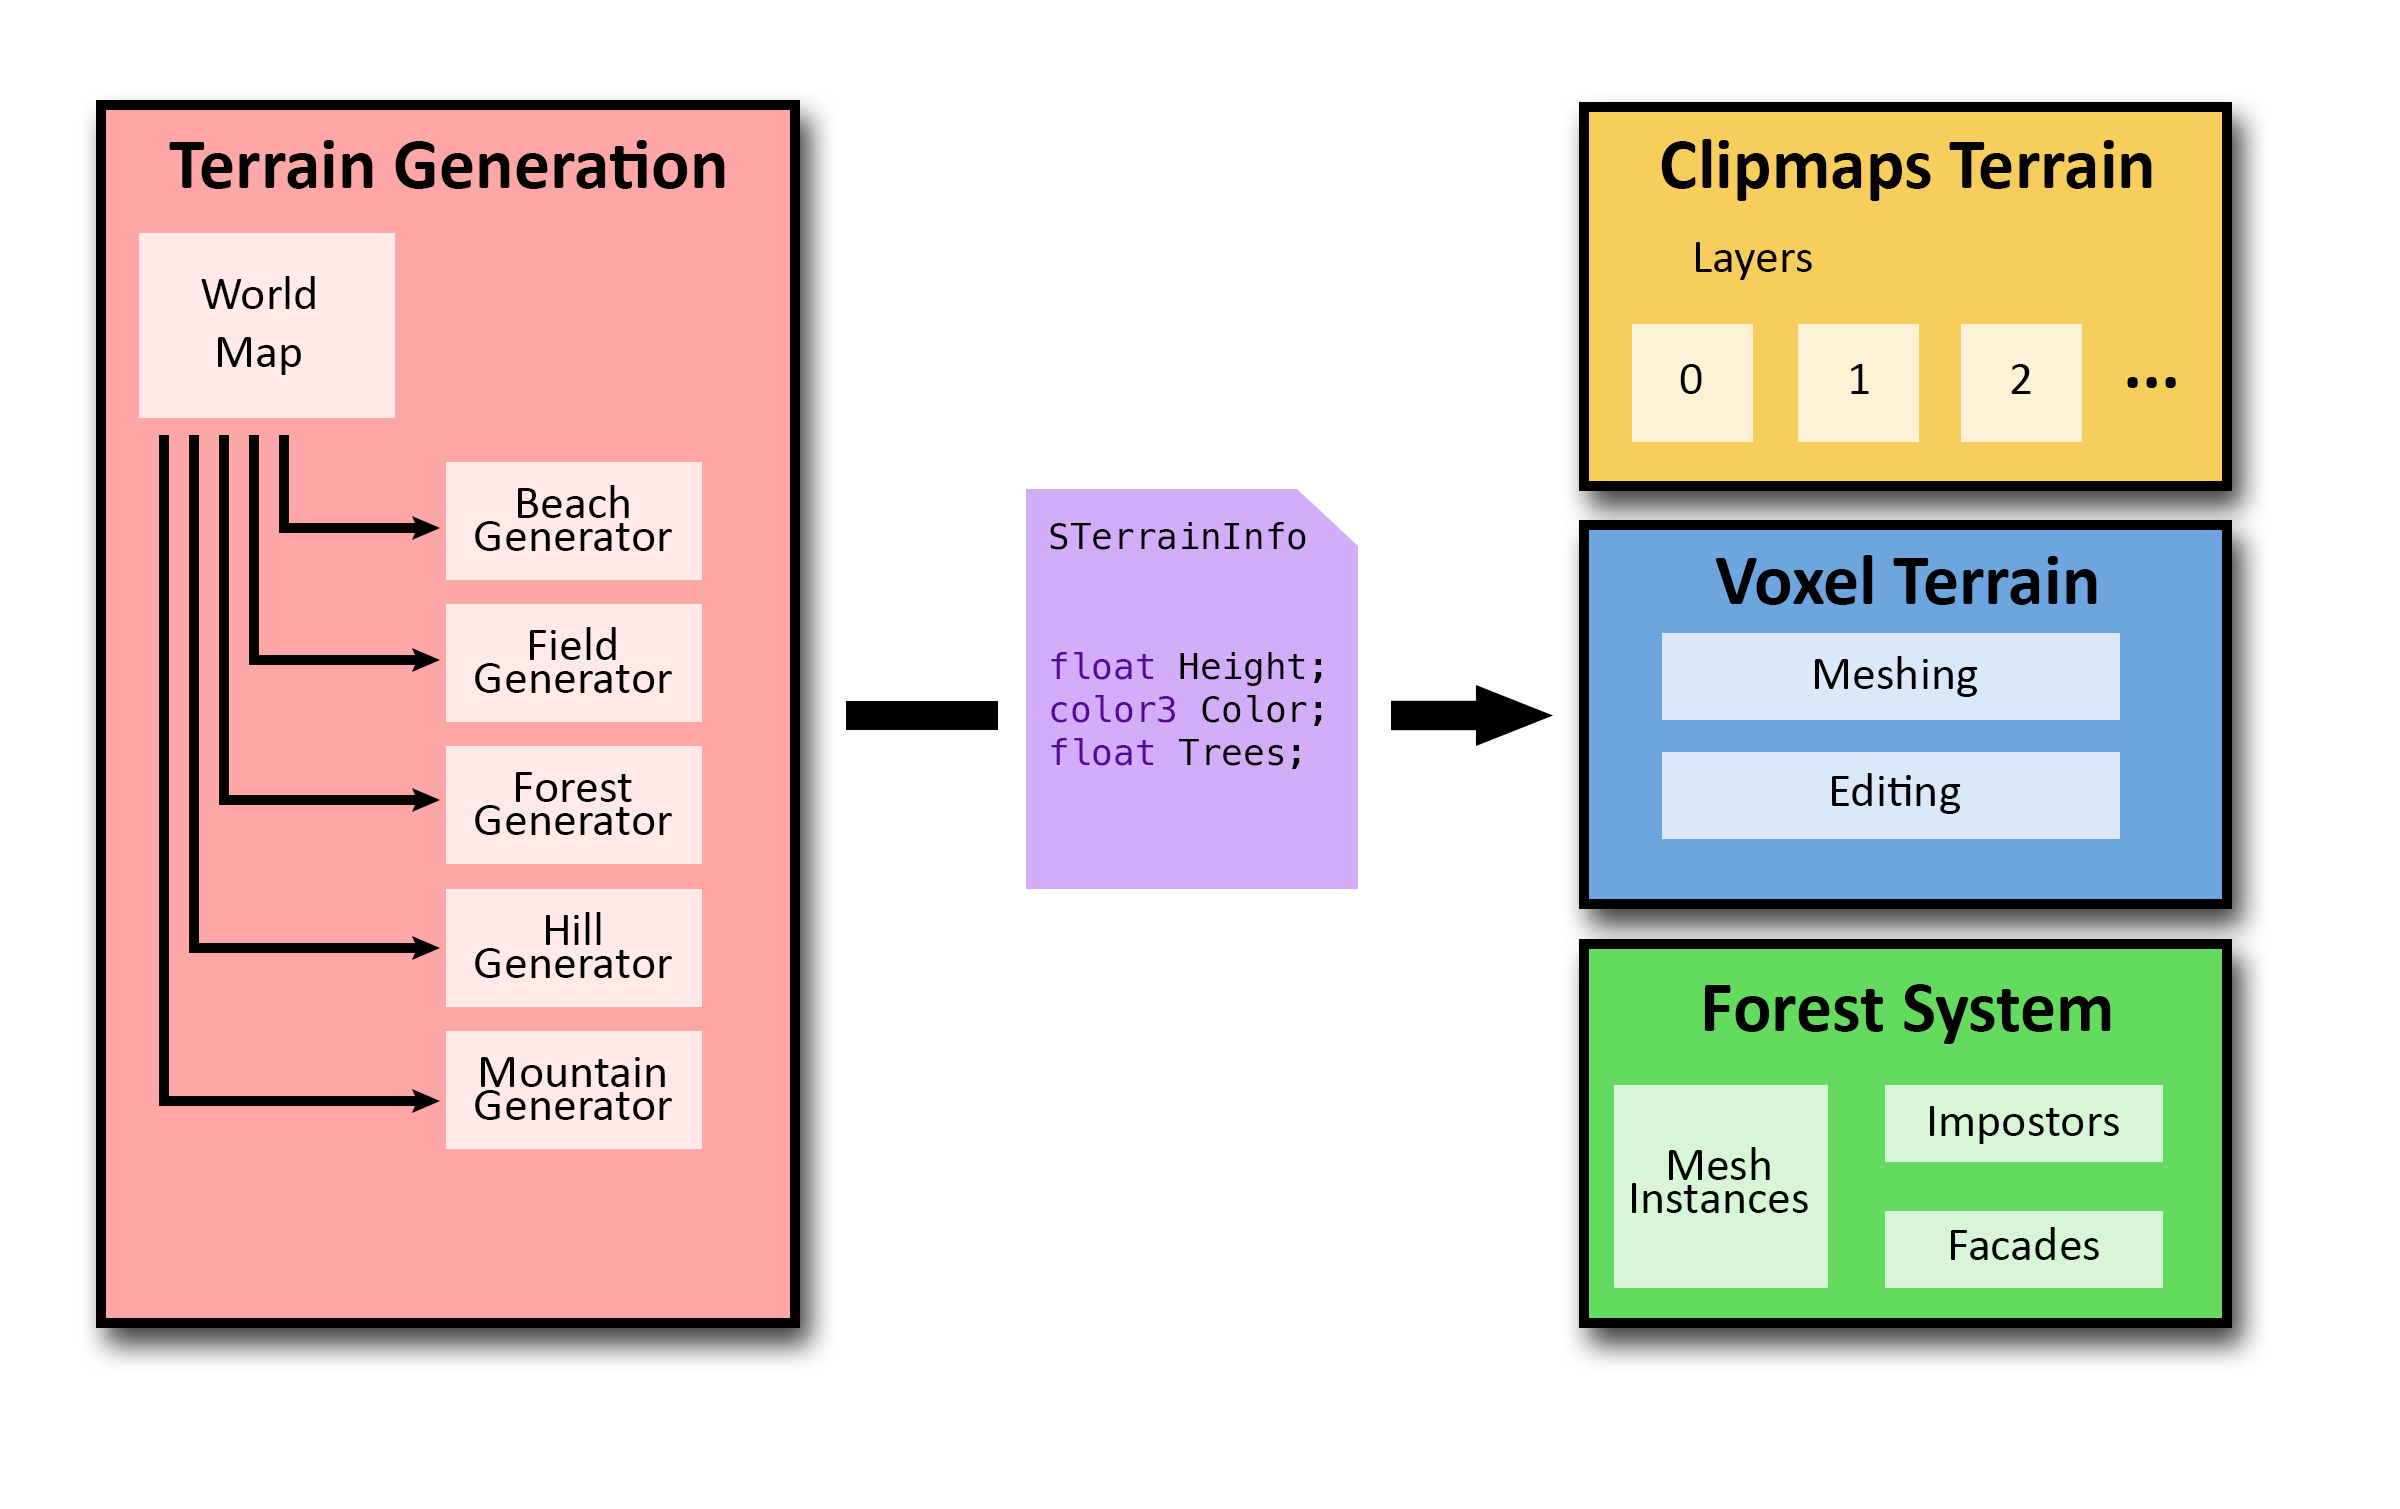
\includegraphics[width=1.0\textwidth]{figures/SystemDiagram.png}
  \caption{Overview of the presented system}
  \label{fig:system1}
\end{figure}


\section{Outline}

In Chapter \ref{bgrnd} we discuss some of the terrain rendering and generation techniques that form the basis for our system.
Then, in Chapter \ref{rworks} we compare some similar systems to the capabilities of Relic.
In Chapters \ref{generation} and \ref{rendering} we describe the contributions of this thesis.
Chapter \ref{results} contains the performance validation of each rendering system, and Chapter \ref{futurework} outlines potential future improvements for the engine.
